\documentclass[11pt]{article}

% ---- Packages ----
\usepackage[utf8]{inputenc}
\usepackage{amsmath,amsfonts,amssymb}
\usepackage{microtype}
\usepackage{geometry}
\usepackage{fancyhdr}
\usepackage{sectsty}

\usepackage{libertine}
\usepackage{booktabs}       % professional-quality tables
\usepackage{nicefrac}       % compact symbols for 1/2, etc.
\usepackage{mathtools}
\mathtoolsset{showonlyrefs}

% nice looking math and font
\usepackage{palatino}
\usepackage{mathpazo}

% For links and references
\usepackage{hyperref}
\usepackage{xcolor}
\definecolor{darkblue}{rgb}{0.0,0.0,0.65}
\definecolor{darkred}{rgb}{0.68,0.05,0.0}
\definecolor{darkgreen}{rgb}{0.0,0.29,0.29}
\definecolor{darkpurple}{rgb}{0.47,0.09,0.29}
\definecolor{darkpink}{rgb}{0.9,0.17,0.31}

\hypersetup{
   colorlinks = true,
   citecolor  = darkblue,
   linkcolor  = darkpink,
   filecolor  = darkgreen,
   urlcolor   = darkpink,
 }

% for generating random text
\usepackage{lipsum}

% FILL REQUIRED INFO
\newcommand{\yourname}{Adarsh Barik} % your name
\newcommand{\lectnum}{1} % Lecture number
\newcommand{\lectdate}{August 14,2025}

% DO NOT CHANGE THIS - START

% ---- Page Setup ----
\geometry{letterpaper, margin=1in}
\setlength{\parskip}{0.8em}
\setlength{\parindent}{0pt}

% ---- Fonts ----
\renewcommand{\sfdefault}{phv} % helvetica-like
\renewcommand{\rmdefault}{ptm} % times-like

% ---- Section style (NeurIPS inspired) ----
\sectionfont{\Large\bfseries}
\subsectionfont{\normalsize\bfseries}

% ---- Header/Footer ----
\pagestyle{fancy}
\fancyhf{} % clear all

% Left header: Instructor + Scriber
\lhead{\textbf{Instructor:} Adarsh Barik\\\textbf{Scribed by:} \yourname{}}

% Right header: Course + Date
\rhead{Lecture \lectnum{}, COV878\\\lectdate{}}

% Center footer: page number
\cfoot{\thepage}

% ---- Title ----
\newcommand{\scribetitle}[1]{
  \begin{center}
    {\LARGE \textsc{Lecture \lectnum{}: #1}} % smart caps
  \end{center}
  \vspace{1em}
  \vskip -\parskip
  \hrule 
  \vskip 0.09in%
}

\AtEndDocument{%
  % Place disclaimer at absolute bottom of final page (flush to bottom)
  \vspace*{\fill}
  \noindent%
  \color{gray}
  \rule{\linewidth}{0.5pt}
  \smallskip
  \textbf{Disclaimer:} These notes have not been scrutinized with the level of rigor usually applied to formal publications. Readers should verify the results before use.
}
% DO NOT CHANGE THIS - END

% Used Defined Packages
\usepackage{tikz}
\usepackage{tcolorbox}
\usepackage{amsthm}
\usepackage{bigints}

\newtheorem{theorem}{Theorem}
\newtheorem{corollary}{Corollary}
\newtheorem{question}{Question}
\newtheorem{lemma}{Lemma}

\newcommand{\real}{\mathbb{R}}
\newcommand{\E}[1]{\mathbb{E}\left[ #1 \right]}
\newcommand{\prob}[1]{\mathbb{P}\left[ #1 \right]}
\newcommand{\var}[1]{\mathbb{V}\text{ar}\left[ #1 \right]}
\newcommand{\given}{\,\middle\vert\,}
\newcommand{\abs}[1]{\left| #1 \right|}
\newcommand{\calX}{\mathcal{X}}

% ---- Document ----
\begin{document}

\scribetitle{Markov's Inequality and Applications}

% \section{Introduction}
% \label{sec:introduction}

In this course, we will focus on establishing rigorous performance guarantees for machine learning (ML) algorithms. These guarantees are commonly expressed through generalization bounds, sample complexity estimates, convergence rates, etc. To derive such results, we typically leverage the statistical properties inherent to the problem setting.

A typical ML pipeline can be modeled as follows:

\begin{tcolorbox}
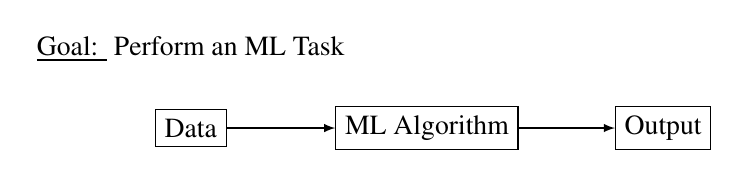
\begin{tikzpicture}
    \node[] at (0, 0) {\underline{Goal: } Perform an ML Task};
    \node[draw] (a) at (0, -1) {Data};
    \node[draw] (b) at (3, -1) {ML Algorithm};
    \node[draw] (c) at (6, -1) {Output};
    \draw[-latex] (a) -- (b);
    \draw[-latex] (b) -- (c);
\end{tikzpicture}
\end{tcolorbox}

Consider the following instantiation of this setup.
\begin{enumerate}
    \item \emph{Goal:} We want to estimate the mean of a Gaussian distribution.
    \item \emph{Data:} We draw $n$ i.i.d. samples $x_1,\ldots,x_n$ from a one-dimensional Gaussian distribution with (unknown) mean $\mu$ and variance $\sigma^2$, i.e., $x_i \underset{\text{i.i.d.}}\sim \mathcal{N}(\mu, \sigma^2),\; \forall i \in \{1,\ldots,n\}$.
    \item \emph{ML Algorithm:} We simply take an average of the $n$ samples.
    \item \emph{Output:} The final output is given by $\hat{\mu}$, where 
    \begin{align}
        \hat{\mu} = \frac{1}{n} \sum_{i=1}^n x_i~.
    \end{align}
\end{enumerate}
We would like $\hat{\mu}$ to be a good estimate of $\mu$. To that end, we ask the following precise question:
\begin{tcolorbox}
\begin{question}[Estimating Mean of a Gaussian random variable]
    \label{question:gaussian mean}
    Given an $\epsilon > 0$ and $\delta > 0$, how many i.i.d. samples are sufficient to ensure that $| \hat{\mu} - \mu | \leq \epsilon$ with probability at least $1 - \delta$?
\end{question}
\end{tcolorbox}
In this lecture, we will see how Markov's inequality, a fundamental result in probability theory, can be used to answer this question.

\section{Some Probability Basics}

Consider a random variable $x$ with support on $\mathcal{X}$ and probability density function $p(\cdot)$. Let $f:\mathcal{X} \to \mathbb{R}$ be a function of the random variable $x$. Then,
\begin{align}
    \label{eq: expectation of a function}
    \E{f(x)} = \int_{x \in \calX} f(x) p(x) dx~.
\end{align}

If we choose $f(x) = (x - \E{x})^2$, we obtain the definition of the variance of $x$, given by $\var{x} = \E{(x - \E{x})^2}$. Another important example is $f(x) = \mathbb{1}_A(x)$, the indicator function for an event $A$, which is defined as 

\begin{align}
    f(x) = \mathbb{1}_A(x) = \begin{cases}
        1, \; x \in A \\
        0, \; \text{otherwise}
    \end{cases}~.
\end{align}
Note that $\prob{A} = \int_{x \in A} p(x) dx = \int_{x \in \calX} \mathbb{1}_A(x) p(x) dx = \E{\mathbb{1}_A(x)}$.

\section{Markov's Inequality}

Next, we will present Markov's inequality for a non-negative random variable $x$.
\begin{theorem}[Markov's inequality]
    \label{thm:markov's inequality}
    Let $x$ be a non-negative random variable with probability density function $p(\cdot)$. For any fixed $a > 0$, we have that
    \begin{align}
        \label{eq:markov's inequality}
        \prob{x \geq a} \leq \frac{\E{x}}{a}~.
    \end{align}
\end{theorem}
\begin{proof}
    We begin by the definition of $\E{x}$.
    \begin{align}
        \E{x} &= \int_{0}^\infty x p(x) dx \\
        &= \underbrace{\int_{0}^a x p(x) dx}_{\geq 0} + \int_{a}^\infty x p(x) dx \\
        &\geq \int_{a}^\infty x p(x) dx \\
        &\geq a\int_{a}^\infty  p(x) dx\\
        &= a \prob{x \geq a}
    \end{align}
\end{proof}
We get Chebyshev's inequality as an immediate consequence of Markov's inequality.
\begin{corollary}[Chebyshev's inequality]
    \label{thm:chebyshev's inequality}
    Let $x$ be a random variable with probability density function $p(\cdot)$. For any fixed $a > 0$, we have that
    \begin{align}
        \label{eq:chebyshev's inequality}
        \prob{\abs{x - \E{x}} \geq a} \leq \frac{\var{x}}{a^2}~.
    \end{align}
\end{corollary}
\begin{proof}
    The proof is left as an exercise.
\end{proof}
Chebyshev's inequality immediately gives us a way to answer Question \ref{question:gaussian mean}. Consider 
\begin{align}
    z &= \frac{1}{n} \sum_{i=1}^n x_i = \hat{\mu} \\
    \E{z} &= \mu \\
    \var{z} &= \frac{\sigma^2}{n}~.
\end{align}
Using Chebyshev's inequality~\eqref{eq:chebyshev's inequality}, it follows that
\begin{align}
    \prob{\abs{z - \E{z}} \geq \epsilon} = \prob{\abs{\hat{\mu} - \mu} \geq \epsilon} \leq \frac{\sigma^2}{n \epsilon^2}~.
\end{align}
Taking $n \geq \frac{\sigma^2}{\delta \epsilon^2}$ provides an answer to  Question~\ref{question:gaussian mean}. While this bound is valid, it does not exploit any specific distributional properties of the $x_i$'s. Next, we will demonstrate that by leveraging the fact that the $x_i$'s are i.i.d. Gaussian random variables, we can obtain significantly improved sample complexity bounds.

\section{Concentration Inequalities for the Mean of Gaussian Random Variables}

Recall that two random variables $x$ and $y$ with supports $\calX$ and $\mathcal{Y}$ and probability density functions $p_x(\cdot)$ and $p_y(\cdot)$ respectively are independent if and only if their joint probability density function $p_{xy}(\cdot,\cdot)$ decomposes as:
\begin{align}
    \label{eq:independence}
    p_{xy}(x, y) = p_x(x) p_y(y),\; \forall x \in \calX, y \in \mathcal{Y}~.
\end{align}
Equation~\eqref{eq:independence} leads to the following result.

\begin{lemma}
    \label{lem:independent functions}
    Let $x$ and $y$ be two independent random variables with supports on $\calX$ and $\mathcal{Y}$. For two arbitrary functions $f:\calX \to \real$ and $g:\mathcal{Y} \to \real$, we have that:
    \begin{align}
        \label{eq: independent functions}
        \E{f(x)g(y)} = \E{f(x)}\E{g(y)}~.
    \end{align}
\end{lemma}
\begin{proof}
    The proof is left as an exercise.
\end{proof}
Now we are ready to prove the following stronger result:
\begin{theorem}
    \label{thm: one sided gaussian bound}
    Let $x_1,\ldots,x_n$ are $n$ independent standard Gaussian random variables, i.e., $x_i \underset{\text{i.i.d.}}\sim \mathcal{N}(0, 1),\; \forall i \in \{1,\ldots,n\}$. Then, for any fixed $\epsilon > 0$, we have that:
    \begin{align}
        \label{eq: one sided gaussian bound}
        \prob{\frac{1}{n} \sum_{i=1}^n x_i \geq \epsilon} \leq \exp\left( \frac{-n\epsilon^2}{2} \right)~.
    \end{align}
\end{theorem}
\begin{proof}
    Pick some arbitrary $t > 0$. We will set an appropriate $t$ later in the proof.
    \begin{align}
         \prob{\frac{1}{n} \sum_{i=1}^n x_i \geq \epsilon} &=  \prob{ \sum_{i=1}^n x_i \geq n\epsilon} \\
         &=  \prob{ \exp\left(t\sum_{i=1}^n x_i \right) \geq \exp\left(tn\epsilon\right)} \label{eq: nonnegative t and exp}\\
         &\leq \frac{\E{\exp\left(t\sum_{i=1}^n x_i \right)}}{\exp\left(tn\epsilon\right)} \label{eq: markov}\\
         &= \frac{\E{\prod_{i=1}^n\exp\left(t x_i \right)}}{\exp\left(tn\epsilon\right)} \label{eq: sum to prod}\\
         &= \frac{\prod_{i=1}^n\E{\exp\left(t x_i \right)}}{\exp\left(tn\epsilon\right)} \label{eq: independence}
    \end{align}
    where \eqref{eq: nonnegative t and exp} follows due to non-negativity of $t$ and $\exp(\cdot)$, \eqref{eq: markov} uses Markov's inequality, and \eqref{eq: independence} holds due to \eqref{eq: independent functions}. Furthermore, recall that $x_i$'s are independent draws of standard Gaussian random variable (denoted as $x$ below) with probability density function $p(x) = \frac{\exp\left( \frac{-x^2}{2}\right)}{\sqrt{2\pi}}$. Therefore,  
    \begin{align}
         \prob{\frac{1}{n} \sum_{i=1}^n x_i \geq \epsilon} &\leq \frac{\left(\E{\exp\left(t x \right)}\right)^n}{\exp\left(tn\epsilon\right)} \label{eq: iid}\\
         &=\frac{\left(\bigints_{-\infty}^\infty \exp\left(tx\right) \frac{\exp\left( \frac{-x^2}{2}\right)}{\sqrt{2\pi}} dx \right)^n}{\exp\left(tn\epsilon\right)} \label{eq: integration}\\
          &=\frac{\left( \exp\left(\frac{t^2}{2}\right) \right)^n}{\exp\left(tn\epsilon\right)} \label{eq: integration ans}\\
          &= \exp\left(\frac{nt^2}{2} - nt\epsilon  \right) \label{eq: final}
    \end{align}
    We observe that right hand side is minimized by choosing $t = \epsilon$. We complete the proof by plugging it back in \eqref{eq: final}.
\end{proof}

Theorem~\ref{thm: one sided gaussian bound} provides a one-sided bound on the mean of standard Gaussian random variables. However, to fully address Question~\ref{question:gaussian mean}, a two-sided bound is needed. We apply a union bound technique to derive the desired two-sided result.

\begin{lemma}[Union bound]
    \label{lem:union bound}
    Let $A$ and $B$ be two events that depend on the random variable $x$. Then
    \begin{align}
        \label{eq: union bound}
        \prob{A(x) \;\text{or}\; B(x) } \leq \prob{A(x)} + \prob{B(x)}~. 
    \end{align}
\end{lemma}
\begin{proof}
    The proof is left as an exercise.
\end{proof}
Lemma~\ref{lem:union bound} along with Theorem~\ref{thm: one sided gaussian bound} leads to the following result.
\begin{theorem}
    \label{thm: two sided gaussian bound}
    Let $x_1,\ldots,x_n$ be $n$ independent standard Gaussian random variables. For any choice of $\epsilon > 0$ and $\delta > 0$, let $n \geq \frac{2 \log \frac{2}{\delta}}{\epsilon^2}$. Then,
    \begin{align}
        \label{eq: two sided gaussian bound}
        \prob{\abs{\frac{1}{n} \sum_{i=1}^n x_i} \leq \epsilon} \geq 1 -  \delta~.
    \end{align}
\end{theorem}
\begin{proof}
    \begin{align}
        \prob{\abs{\frac{1}{n} \sum_{i=1}^n x_i} \leq \epsilon} &= \prob{ \frac{1}{n} \sum_{i=1}^n x_i \leq \epsilon \; \text{and}\; \frac{1}{n} \sum_{i=1}^n x_i \geq -\epsilon} \\
        &= 1 - \prob{ \frac{1}{n} \sum_{i=1}^n x_i > \epsilon \; \text{or}\; \frac{1}{n} \sum_{i=1}^n x_i < -\epsilon}
    \end{align}
    We observe that $x$ is a standard Gaussian random variable and so is $-x$. Moreover, using Lemma~\ref{lem:union bound} and Theorem~\ref{thm: one sided gaussian bound}, we have:
    \begin{align}
        \prob{ \frac{1}{n} \sum_{i=1}^n x_i > \epsilon \; \text{or}\; \frac{1}{n} \sum_{i=1}^n x_i < -\epsilon} &\leq \prob{ \frac{1}{n} \sum_{i=1}^n x_i \geq \epsilon \; \text{or}\; \frac{1}{n} \sum_{i=1}^n x_i \leq -\epsilon} \\
        &\leq \prob{ \frac{1}{n} \sum_{i=1}^n x_i \geq \epsilon}  + \prob{\frac{1}{n} \sum_{i=1}^n x_i \leq -\epsilon} \\
        &= \prob{ \frac{1}{n} \sum_{i=1}^n x_i \geq \epsilon}  + \prob{\frac{1}{n} \sum_{i=1}^n - x_i \geq \epsilon} \\
        &\leq 2 \exp\left(\frac{-n\epsilon^2}{2}\right)~.
    \end{align}
    We finish the proof by picking $\delta \geq 2 \exp\left(\frac{-n\epsilon^2}{2}\right)$.
\end{proof}
Extending results for the standard Gaussian random variables to the general Gaussian distribution random variables is straightforward. Specifically, the following result holds:
\begin{corollary}
    \label{cor: general gaussian two-sided}
     Let $x_1,\ldots,x_n$ be $n$ independent Gaussian random variables with mean $\mu$ and variance $\sigma^2$. For any choice of $\epsilon > 0$ and $\delta > 0$, let $n \geq \frac{2 \sigma^2 \log \frac{2}{\delta}}{\epsilon^2}$. Then,
    \begin{align}
        \prob{\abs{\frac{1}{n} \sum_{i=1}^n x_i - \mu } \leq \epsilon} \geq 1 -  \delta~.
    \end{align}
\end{corollary}
\begin{proof}
    The proof is left as an exercise.
\end{proof}

\end{document}
